\chapter{Módulo: Identidad y Acceso}
\label{mod:01-identidad-y-acceso}

\section{Propósito}
\label{sec:identidad-proposito}

Gestiona quién puede entrar a SIGA y con qué credenciales: autenticación (login JWT), ciclo de vida de la cuenta (\code{User}) y los flujos de contraseña (self-service, reset por admin, cambio obligatorio en primer login, recuperación por email). Es la base sobre la que se apoyan todos los demás módulos --- sin \code{User} autenticado no hay acceso a ningún endpoint protegido. El ABM del catálogo de \code{Role}/\code{Permission} en sí (qué permisos tiene cada rol) se documenta aparte en el \hyperref[mod:12-roles-y-permisos]{Módulo de Roles y Permisos}; aquí el foco es la cuenta y su acceso.

\section{Entidades principales}
\label{sec:identidad-entidades}

Ver Capítulo~\ref{sec:modelo-datos}, Figura~\ref{fig:er-identidad-rbac}.

\begin{longtable}{p{2.8cm}p{10.5cm}}
\caption{Entidades principales del módulo de Identidad y Acceso.}\label{tab:identidad-entidades}\\
\toprule
\textbf{Entidad} & \textbf{Rol} \\
\midrule
\endfirsthead
\toprule
\textbf{Entidad} & \textbf{Rol} \\
\midrule
\endhead
\bottomrule
\endfoot
\code{Person} & Datos personales de cualquier individuo del sistema --- ver Capítulo~\ref{sec:modelo-datos}. \\
\code{User} & Cuenta de acceso, 1:1 con \code{Person}. \code{SucursalId} nullable, \code{PasswordHash}, \code{IsActive}, \code{IsEmailVerified}, \code{Must}\allowbreak \code{Change}\allowbreak \code{Password}, \code{Password}\allowbreak \code{Reset}\allowbreak \code{Token}. \\
\code{Role} / \code{UserRole} & Roles asignados al usuario (many-to-many) --- detalle en el \hyperref[mod:12-roles-y-permisos]{Módulo de Roles y Permisos}. \\
\end{longtable}

\section{Reglas de negocio clave}
\label{sec:identidad-reglas}

\begin{itemize}
  \item \textbf{Login es email más contraseña, resuelto vía \code{Person.Email}} (join \code{User}$\to$\code{Person}), no hay username separado.
  \item \textbf{JWT lleva permisos, no roles} --- el token emite un claim \code{"permission"} por cada permiso resuelto de los roles del usuario, más \code{professional_id} (si aplica) y \code{sucursal_id} (si el usuario tiene sucursal fija). Ver \hyperref[adr:0003]{ADR 0003} y Capítulo~\ref{sec:arch}, \S\ref{sec:arch-autorizacion}.
  \item \textbf{Auto-registro de pacientes es el único flujo de alta pública} (\code{POST /api/auth/}\allowbreak \code{register/patient}): protegido con hCaptcha, crea \code{Person}+\code{User}+\code{Patient} con \code{Is}\allowbreak \code{Email}\allowbreak \code{Verified=false} y exige verificar el email (\code{GET /api/auth/verify-email?token=}) antes de poder loguear. El alta de \code{Professional}/\code{Empleado} (por un admin) \textbf{no} pasa por este flujo.
  \item \textbf{\code{Is}\allowbreak \code{Email}\allowbreak \code{Verified=true} bloquea el login si es \code{false}} --- pero solo aplica de verdad al auto-registro público. \code{ProfessionalService.}\allowbreak \code{CreateAsync}/\code{EmpleadoService.}\allowbreak \code{CrearAsync} setean \code{Is}\allowbreak \code{Email}\allowbreak \code{Verified=true} directamente al crear la cuenta, porque son altas ``vouched-for'' por un admin y no necesitan verificar email.
  \item \textbf{\code{Must}\allowbreak \code{Change}\allowbreak \code{Password} solo aplica a cuentas nuevas, no retroactivo.} Se setea \code{true} al crear un \code{Professional}/\code{Empleado}; no bloquea el login (a diferencia de \code{IsEmailVerified}) --- el frontend redirige \emph{después} de autenticar, vía guard de router que cubre navegación directa y refresh, no solo el submit del login. Ver \hyperref[adr:0012]{ADR 0012}.
  \item \textbf{Tres formas de cambiar contraseña, cada una con su propio permiso/regla:} self-service (\code{POST /api/auth/change-password}, pide la actual), admin-reset (\code{PUT /api/users/{id}/reset-password}, policy \code{editar_usuario}, no pide la actual, fuerza \code{Must}\allowbreak \code{Change}\allowbreak \code{Password=true}), y recuperación por email sin sesión (\code{forgot-password}/\code{reset-password}, \code{AllowAnonymous}, con token).
  \item \textbf{Borrado lógico vía \code{User.}\allowbreak \code{IsActive=false}}, no hay borrado físico de cuentas.
\end{itemize}

\section{Endpoints}
\label{sec:identidad-endpoints}

Detalle completo (policies, DTOs) en el Apéndice de Referencia de API, \S\ref{sec:api-identidad}.

\begin{longtable}{p{1.6cm}p{5.6cm}p{6.2cm}}
\caption{Endpoints principales del módulo de Identidad y Acceso.}\label{tab:identidad-endpoints}\\
\toprule
\textbf{Método} & \textbf{Ruta} & \textbf{Descripción} \\
\midrule
\endfirsthead
\toprule
\textbf{Método} & \textbf{Ruta} & \textbf{Descripción} \\
\midrule
\endhead
\bottomrule
\endfoot
POST & \code{/}\allowbreak \code{api/}\allowbreak \code{auth/}\allowbreak \code{register/}\allowbreak \code{patient} & Auto-registro público de paciente (hCaptcha más verificación de email) \\
GET & \code{/}\allowbreak \code{api/}\allowbreak \code{auth/}\allowbreak \code{verify-email} & Confirma el email desde el link enviado \\
POST & \code{/api/auth/login} & Login, devuelve JWT más claims \\
POST & \code{/}\allowbreak \code{api/}\allowbreak \code{auth/}\allowbreak \code{change-password} & Self-service, requiere contraseña actual \\
POST & \code{/}\allowbreak \code{api/}\allowbreak \code{auth/}\allowbreak \code{forgot-password} / \code{reset-password} & Recuperación sin sesión, por token de email \\
GET / DELETE & \code{/api/users} & Listado y desactivación de cuentas \\
PUT & \code{/api/users/{id}/}\allowbreak \code{reset-password} & Reset por admin, sin pedir la actual \\
\end{longtable}

\section{Flujo típico}
\label{sec:identidad-flujo}

\subsection{Auto-registro de paciente y verificación de email}

\begin{figure}[htbp]
\centering
\begin{tikzpicture}
  \node[actor] (fe) at (0,0) {SIGA-Web\\\footnotesize RegisterView};
  \node[actor] (api) at (3.4,0) {AuthController};
  \node[actor] (hc) at (6.6,0) {hCaptcha};
  \node[actor] (db) at (9.6,0) {PostgreSQL};
  \node[actor] (rs) at (12.6,0) {Resend};

  \draw[lineavida] (fe.south) -- ++(0,-6.5);
  \draw[lineavida] (api.south) -- ++(0,-6.5);
  \draw[lineavida] (hc.south) -- ++(0,-6.5);
  \draw[lineavida] (db.south) -- ++(0,-6.5);
  \draw[lineavida] (rs.south) -- ++(0,-6.5);

  \draw[mensaje] ($(fe.south)+(0,-0.8)$) -- node[above,font=\scriptsize,align=center]{POST /auth/register/patient\\(datos + captchaToken)} ($(api.south)+(0,-0.8)$);
  \draw[mensaje] ($(api.south)+(0,-1.9)$) -- node[above,font=\scriptsize]{validar captchaToken} ($(hc.south)+(0,-1.9)$);
  \draw[mensajeretorno] ($(hc.south)+(0,-2.6)$) -- node[below,font=\scriptsize]{OK} ($(api.south)+(0,-2.6)$);
  \draw[mensaje] ($(api.south)+(0,-3.6)$) -- node[above,font=\scriptsize,align=center]{crea Person + User\\(IsEmailVerified=false) + Patient} ($(db.south)+(0,-3.6)$);
  \draw[mensaje] ($(api.south)+(0,-4.8)$) -- node[above,font=\scriptsize]{enviar email con link} ($(rs.south)+(0,-4.8)$);
  \draw[mensajeretorno] ($(api.south)+(0,-5.8)$) -- node[below,font=\scriptsize]{200 OK (sin loguear)} ($(fe.south)+(0,-5.8)$);
\end{tikzpicture}
\caption{Auto-registro público de paciente: alta con \texttt{IsEmailVerified=false} y envío del email de verificación.}
\label{fig:seq-registro-paciente}
\end{figure}

\begin{figure}[htbp]
\centering
\begin{tikzpicture}
  \node[actor] (fe) at (0,0) {SIGA-Web};
  \node[actor] (api) at (4,0) {AuthController};
  \node[actor] (db) at (8,0) {PostgreSQL};

  \draw[lineavida] (fe.south) -- ++(0,-3.2);
  \draw[lineavida] (api.south) -- ++(0,-3.2);
  \draw[lineavida] (db.south) -- ++(0,-3.2);

  \node[font=\scriptsize\itshape, align=center] at (4,-0.9) {usuario hace click en el link del email};
  \draw[mensaje] ($(fe.south)+(0,-1.6)$) -- node[above,font=\scriptsize]{GET /auth/verify-email?token=...} ($(api.south)+(0,-1.6)$);
  \draw[mensaje] ($(api.south)+(0,-2.3)$) -- node[above,font=\scriptsize]{User.IsEmailVerified = true} ($(db.south)+(0,-2.3)$);
  \draw[mensajeretorno] ($(api.south)+(0,-2.9)$) -- node[below,font=\scriptsize]{200 OK -- ya puede loguear} ($(fe.south)+(0,-2.9)$);
\end{tikzpicture}
\caption{Verificación de email: continuación del flujo de auto-registro tras el click en el enlace enviado por Resend.}
\label{fig:seq-verificacion-email}
\end{figure}

\subsection{Cambio de contraseña obligatorio (cuenta nueva de staff)}

\begin{figure}[htbp]
\centering
\begin{tikzpicture}
  \node[actor] (admin) at (0,0) {Admin};
  \node[actor] (api) at (3.6,0) {Professional/\\EmpleadoService};
  \node[actor] (u) at (7.6,0) {Nuevo\\profesional/empleado};
  \node[actor] (fe) at (11.4,0) {SIGA-Web\\\footnotesize router guard};

  \draw[lineavida] (admin.south) -- ++(0,-6.5);
  \draw[lineavida] (api.south) -- ++(0,-6.5);
  \draw[lineavida] (u.south) -- ++(0,-6.5);
  \draw[lineavida] (fe.south) -- ++(0,-6.5);

  \draw[mensaje] ($(admin.south)+(0,-0.8)$) -- node[above,font=\scriptsize]{crear Professional/Empleado} ($(api.south)+(0,-0.8)$);
  \node[font=\scriptsize\itshape, align=center, text width=3.6cm] at (3.6,-1.7) {User.MustChangePassword=true\\IsEmailVerified=true};
  \draw[mensaje] ($(u.south)+(0,-2.6)$) -- node[above,font=\scriptsize]{login con contraseña temporal} ($(fe.south)+(0,-2.6)$);
  \node[font=\scriptsize\itshape, align=center, text width=3.4cm] at (11.4,-3.4) {guard detecta\\mustChangePassword=true};
  \draw[mensaje] ($(fe.south)+(0,-4.2)$) -- node[above,font=\scriptsize,align=center]{redirige a /cambiar-contrasena\\(bloquea el resto de la app)} ($(u.south)+(0,-4.2)$);
  \draw[mensaje] ($(u.south)+(0,-5.2)$) -- node[above,font=\scriptsize]{POST /auth/change-password} ($(api.south)+(0,-5.2)$);
  \node[font=\scriptsize\itshape] at (3.6,-5.8) {User.MustChangePassword=false};
  \draw[mensajeretorno] ($(fe.south)+(0,-6.3)$) -- node[below,font=\scriptsize]{navegación normal habilitada} ($(u.south)+(0,-6.3)$);
\end{tikzpicture}
\caption{Cambio de contraseña obligatorio: el guard del router intercepta cualquier navegación mientras \texttt{mustChangePassword} sea verdadero.}
\label{fig:seq-cambio-password-obligatorio}
\end{figure}

\section{Vistas de frontend}
\label{sec:identidad-vistas}

\begin{itemize}
  \item \code{LoginView.vue}, \code{RegisterView.vue}, \code{VerifyEmailView.}\allowbreak \code{vue}
  \item \code{OlvideContrasenaView.}\allowbreak \code{vue}, \code{RestablecerContrasenaView.}\allowbreak \code{vue} (recuperación por email)
  \item \code{CambiarContrasena}\allowbreak \code{ObligatoriaView.}\allowbreak \code{vue} (pantalla aislada, forzada por router guard)
  \item \code{UsuariosView.vue} (listado, roles por usuario, activar/desactivar, ``Restablecer contraseña'' en el modal de gestión)
  \item Modal ``Cambiar contraseña'' en \code{AppHeader.vue} (self-service, no es una vista propia)
\end{itemize}

\section{Interfaz}
\label{sec:identidad-interfaz}

\begin{figure}[htbp]
\centering
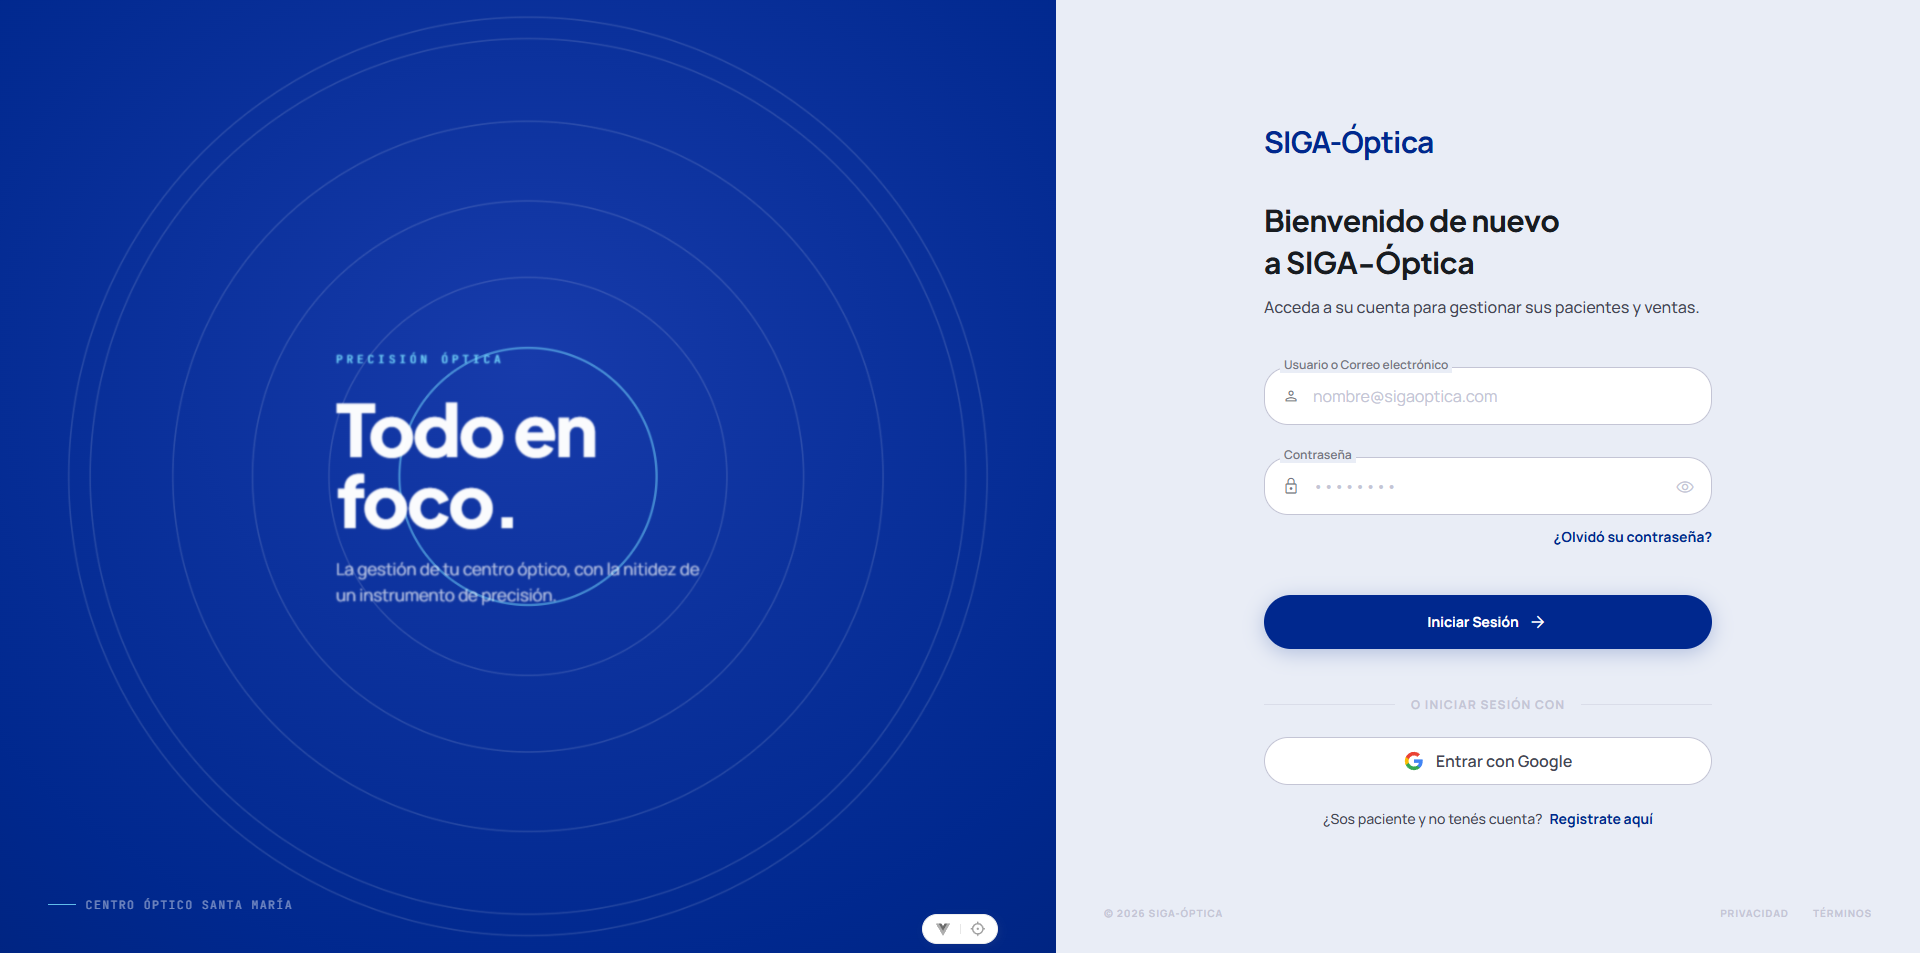
\includegraphics[width=0.95\textwidth]{imagenes/mod01-login.png}
\caption{Pantalla de inicio de sesión de SIGA-Óptica, con acceso alternativo vía Google y enlace de recuperación de contraseña.}
\label{fig:mod01-login}
\end{figure}

\section{Estado}
\label{sec:identidad-estado}

\Implementado, incluida la recuperación de contraseña por email (\code{forgot-password}/\allowbreak \code{reset-password}).
